\chapter{Interfaz gráfica}
\label{cha:gui}
 
Hasta ahora, las herramientas de verificación y minería mostradas en este proyecto utilizaban interfaces de usuario poco amigables para usuarios inexpertos: a través de línea de comandos para la herramienta STLEval; o mediante código fuente en Python para la librería ParetoLib.

En este apartado proponemos un espacio donde el usuario tenga que simplemente adjuntar los fichero de datos y operaciones (o elegir la operación a realizar desde las opciones disponibles) para finalmente poder visualizar y descargar la salida de señales en forma gráfica.
 
\section{Librerías utilizadas}

Para el desarrollo de la parte gráfica de este proyecto hemos hecho uso de las librerías:
\begin{itemize}
\item \href{https://www.qt.io/qt-for-python}{PyQt}
\item Matplotlib
\item Pandas
\item Seaborn
\end{itemize}
 
\subsection{PyQt}
Esta librería está basada en la biblioteca gráfica QT y nos servirá para realizar el diseño de la aplicación. En nuestro caso optamos por un diseño simple de 2 columnas: En la parte izquierda tendremos los botones y opciones para importar los ficheros de señales y la especificación de la operación, además de un espacio adicional para otras operaciones nuevas a implementar en un futuro. Al lado derecho tendremos la visualización de las señales tratadas y la especificación STL importada.

\begin{figure}[htb]
\centering
  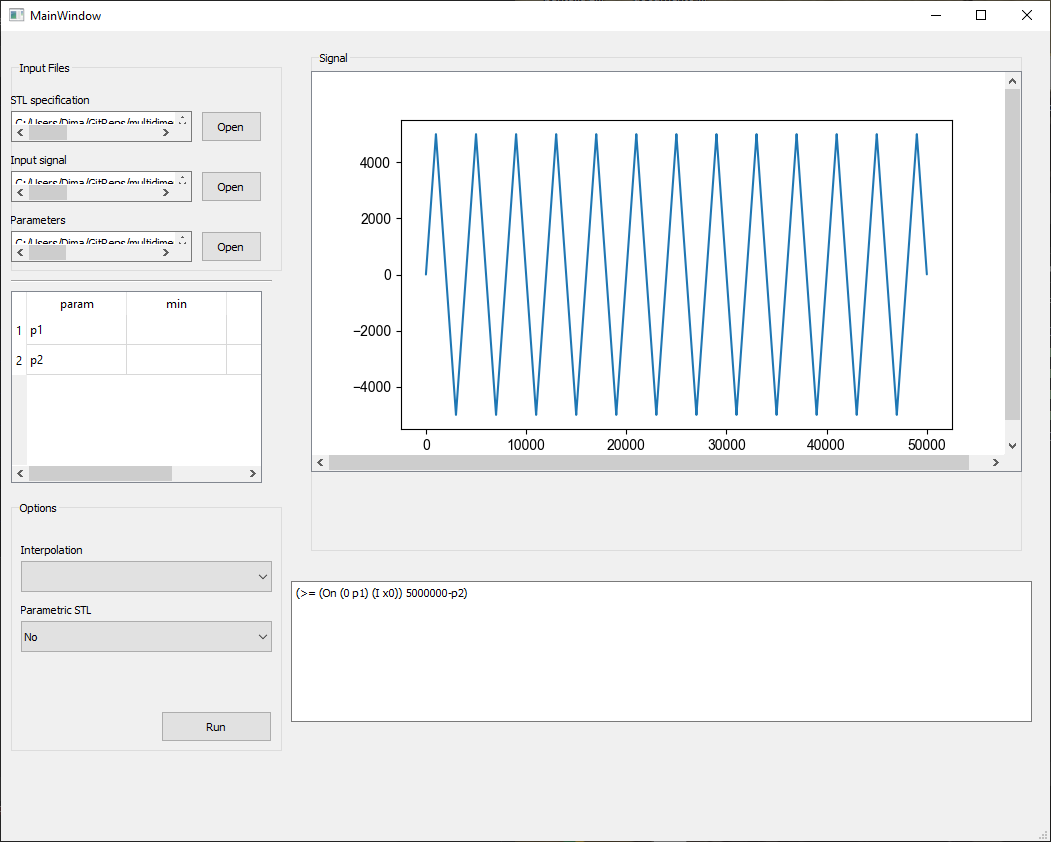
\includegraphics[width=1.0\linewidth]{images/gui} 
\caption{La ventana principal}
\label{fig:gui}
\end{figure}

%Instalación: 
%El desarrollo de la aplicación se hizo en un entorno linux haciendo uso del gestor de paquetes “pip”. 
 
%1 - Antes de todo, tenemos que confirmar la versión de Python que tenemos instalada con ´python3 --version´.
 
%2 - En el caso de que no lo tuviésemos, instalamos el gestor de paquetes “pip” con sudo ‘apt-get install python3-pip’ y actualizamos el mismo ´pip install -U pip´ 
 
%3 - Instalamos la librería PyQT con ´pip install pyqt5´. 
 
\subsection{MatplotLib}
Biblioteca usada para generar gráficos a partir de datos almacenados en un array. Hacemos uso de esta librería con el fin de mostrar las señales resultantes, aplicando las operaciones indicadas, en la sección de la aplicación propuesta para ello. 
 
%Instalación: 
 
%1 - En este caso es sumamente simple realizando: ´sudo apt-get install python3-matplotlib´.
 
\subsection{Pandas}
Librería de Python especializada en el manejo y análisis de estructuras de datos. En nuestro caso usada para la lectura de los ficheros csv, los cuales contienen los datos de entrada de las señales.
 
%Instalación: 
 
%1 - Instalamos la librería con el comando: ´pip install pandas´

\subsection{Seaborn} 
Basada en MatplotLib, es una librería que permite generar fácilmente elegantes gráficos. Nosotros la utilizamos para dibujar señales de los datos leídos de los archivos cvs.
 
%Instalación: 
 
%1 - Instalamos la librería con el comando: ´pip install seaborn´

\section{Estructura}
\begin{figure}[htb]
\centering
  \includegraphics[width=.95\linewidth]{images/uml_diagram} 
\caption{Estructura del proyecto}
\label{fig:est}
\end{figure}
Como vemos en la figura \ref{fig:est}, la GUI se comunica con la librería de minería ParetoLib que nos permite evaluar propiedades con parámetros, utilizando en ese caso los métodos de la librería, o sin ellos, haciendo simplemente una consulta a la API STL. A su vez ParetoLib esta conectado por binarios precomplilados con STL.

La anterior forma de hacer consultas a través de la terminal obligaba a hacerlas por separado a STLe o a la librería de minería dependiendo si quisiésemos una consulta STL paramétrica o no. La nueva GUI unifica el proceso y facilita la usabilidad de cara al usuario.

Como partes aportaciones nuevas al proyecto (marcadas en rojo) esta la propia GUI, los operadores derivada e integral en STLe y una modificación en la API OracleSTLe, con la cual conseguimos que sea factible hacer consultas no paramétricas desde ParetoLib.

\section{Guía de uso}
En esta sección vamos a describir alguna de las partes interactuables o visibles de la GUI:

\begin{itemize}
\item STL specification: Seleccionamos un archivo \textbf{.stl} el cual contiene una formula paramétrica o no, esto es importante porque si deseamos hacer una consulta no paramétrica debemos de ajustar la formula para que no haya ningún parámetro. Cuando seleccionemos el archivo, la descripción de la formula aparecerá en una caja inferior la cual solo sera visual y no modificable.

\item Input signal: Necesita de un archivo \textbf{.csv} que contenga la especificación de la señal. Una vez seleccionado aparece un dibujo de esta en la caja grande de la ventana

\item Parameters: Proporcionamos un archivo \textbf{.param} que contiene los parámetros a estudiar que aparecen en la formula del archivo .stl seleccionado. Al elegir un archivo nos aparecerá mas abajo una caja donde poder rellenar el valor mínimo y máximo de cada parámetro. Para una consulta no paramétrica no hace falta seleccionar ningún archivo.

\item Parametric STL: Elegimos si queremos una consulta STL paramétrica o no, en el caso de quererla seleccionamos que si y viceversa.

\item Run: Boton de ejecutar la consulta. Para poder hacerla necesitamos los 3 input files anteriores descritos (2 en el caso no paramétrico) y se nos devolverá un mapa con las regiones falsas o verdaderas según los parámetros \ref{fig:param} si la consulta es paramétrica o un True/False en el caso contrario. 
\end{itemize} 

\section{Otros}
Cabe mencionar, que para sacar todo el potencial de PyQt5 hemos hecho uso de la herramienta Qt Designer. Gracias a ella hemos podido construir la interfaz en sí. Una vez hecha, la unimos al archivo GUI.py para aportar funcionalidades al propio diseño.
